\documentclass[aspectratio=169]{beamer}
\usepackage[utf8]{inputenc}
\usepackage{transparent}
\usepackage{hyperref}
\usepackage{pgf}
\usepackage{dsfont}
\usepackage{algorithm}
\usepackage{algorithmic}

% here comes my custom theme for university of Bamberg

\logo{\pgfputat{\pgfxy(-1.25,4.25)}{\pgfbox[center,base]{\transparent{0.7} 
\includegraphics[width=.15\textwidth]{uni_bamberg.png}}}}


\newcommand{\nologo}{\setbeamertemplate{logo}{}} % command to set the logo to nothing
\newcommand{\biglogo}{\setbeamertemplate{logo}{\pgfputat{\pgfxy(-2,4)}{\pgfbox[center,base]{ 
\includegraphics[width=.24\textwidth]{uni_bamberg.png}}}}} 

% theming and colors and stuff
\usetheme[progressbar=frametitle, block = fill]{metropolis}
\definecolor{uniblau}{RGB}{4, 66, 119} %#044277
\definecolor{niceorange}{RGB}{255, 128, 0} %#ff8000
\definecolor{nicegray}{RGB}{221, 239, 244} %#ddeff4
\setbeamercolor{palette primary}{bg=uniblau, fg=white}
\setbeamercolor{normal text}{fg=uniblau, bg=white}
\setbeamercolor{itemize item}{fg=niceorange}
\setbeamercolor{itemize subitem}{fg=niceorange}
\setbeamercolor{itemize subsubitem}{fg=niceorange}
\setbeamercolor{enumerate item}{fg=niceorange}
\setbeamercolor{enumerate subitem}{fg=niceorange}
\setbeamercolor{enumerate subsubitem}{fg=niceorange}
\setbeamercolor{block body}{bg=nicegray}
\setbeamercolor{block title}{bg=niceorange,fg=white}
\renewcommand\UrlFont{\color{niceorange}\rmfamily}

% own commands for highlighting
\newcommand{\pop}[1]{{\color{niceorange}\textbf{#1}}}

\def\ps@titlepage{\setbeamertemplate{footline}{}}
\makeatletter
\setbeamertemplate{frame footer}{\tiny{xAI-Proj-M - Model Engineering - B.Bony}}

% custom python style

%title page
\title{Model Engineering -- Dropout v BatchNorm}
\subtitle{Explainable Machine Learning - Deep Learning Life Cycle}
\author{Jonas Amling \and Baptiste Bony \and Benedikt Marsiske}
\institute{University of Bamberg}
\date{\today} 

\begin{document}
% titleframe
{\biglogo
	\setbeamertemplate{footline}{} 
	\begin{frame}{}
		\titlepage
	\end{frame}
}

\begin{frame}{Table of contents}
	\tableofcontents
\end{frame}


{\nologo
\section{Research Question}
	\begin{frame}{Research Question}
    
	Our main Model Engineering challenges:
	\begin{itemize}
		\item Accuracy performance
		\item Prevent overfitting for the model to be generalizable to new data
	\end{itemize}
	Research Question: \pop{Do dropout layers prevent overfitting ?}\\
    \bigskip
    In addition to Dropout, we tried another regularization technique, namely Batch Normalization.\\
	\end{frame}
 

    \begin{frame}{Overfitting}
        \begin{figure}
            \centering
            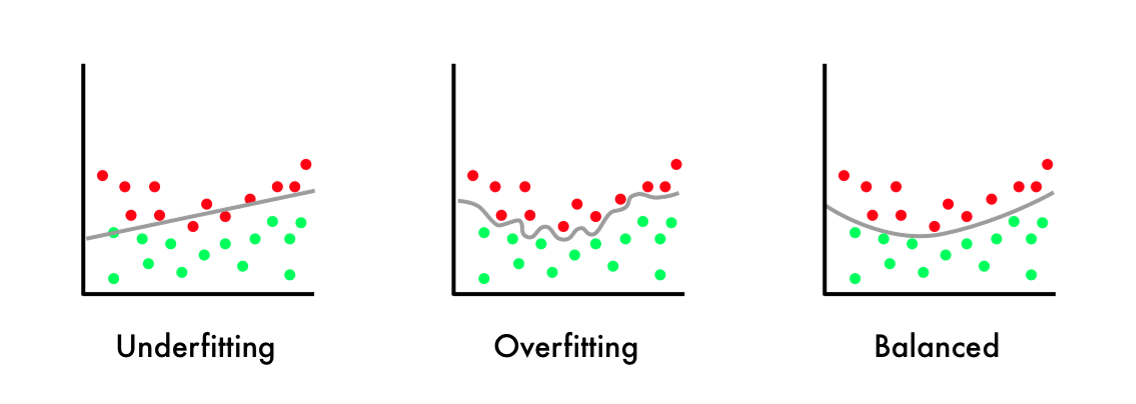
\includegraphics[width=1\textwidth]{img/Overfitting.png}
            \caption{Visual explanation of Overfitting}
        \end{figure}
    \end{frame}

 
\section{Model Engineering Process} 

    \begin{frame}{Overview of the different datasets}
        \begin{figure}
            \centering
            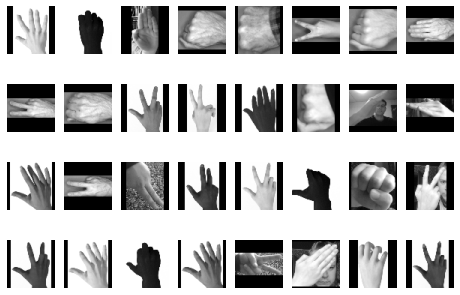
\includegraphics[width=0.6\textwidth]{img/trainloader.png}
            \caption{Sample of the Training Dataset}
        \end{figure}
    \end{frame}

    \begin{frame}{Overview of the different datasets}
        \begin{figure}
            \centering
            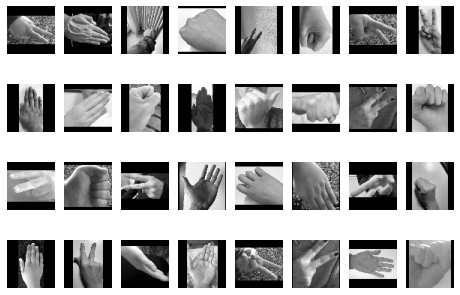
\includegraphics[width=0.6\textwidth]{img/validationloader.png}
            \caption{Sample of the Validation Dataset}
        \end{figure}
    \end{frame}

    \begin{frame}{Overview of the different datasets}
        \begin{figure}
            \centering
            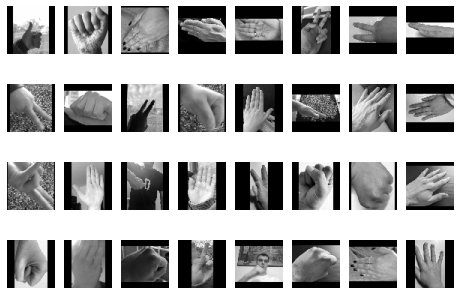
\includegraphics[width=0.6\textwidth]{img/testloader.png}
            \caption{Sample of the Testing Dataset}
        \end{figure}
    \end{frame}
    
    \begin{frame}{Our first model}
        \begin{figure}
            \centering
            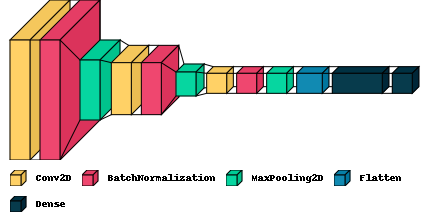
\includegraphics[width=0.6\textwidth]{img/model_without_dropout.png}
            \caption{Visualization of our first model}
        \end{figure}
    \end{frame}


    \begin{frame}{VGG16 \cite{VGG16}}
        \begin{figure}
            \centering
            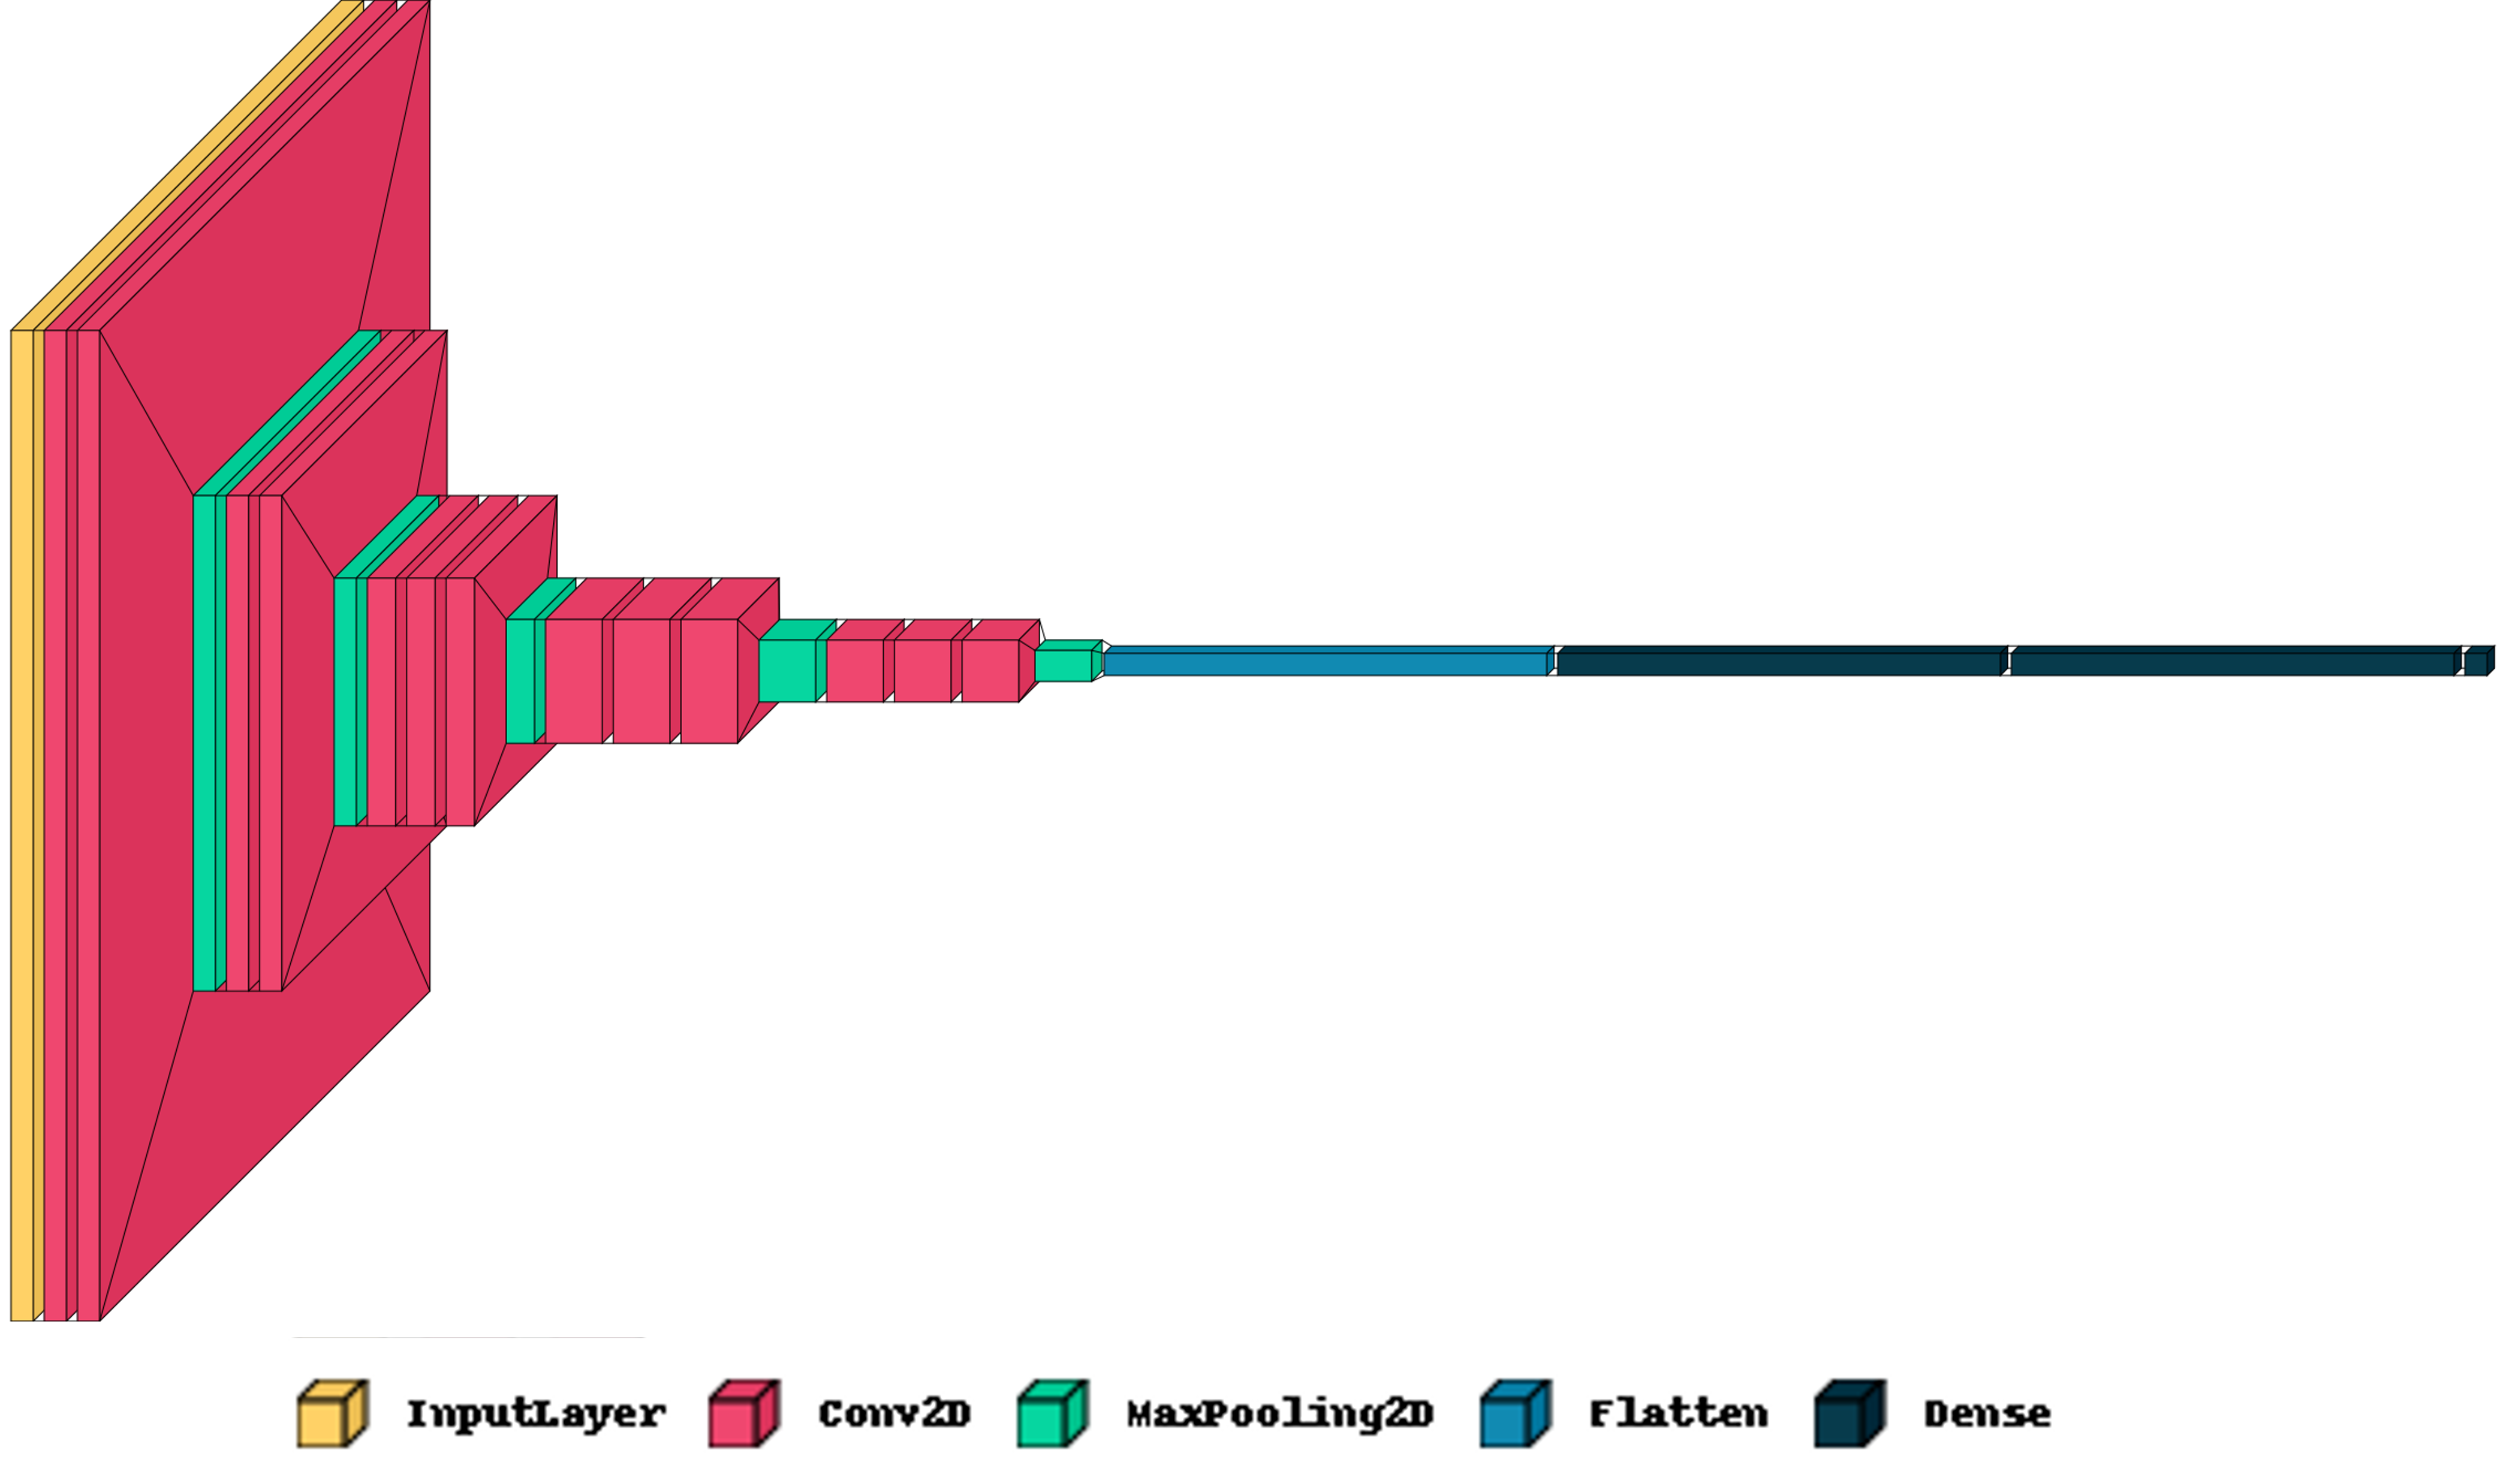
\includegraphics[width=0.6\textwidth]{img/model_VGG16.png}
            \caption{Visualization of the VGG16 model}
        \end{figure}
    \end{frame}

    \begin{frame}{Our custom model}
        \begin{figure}
            \centering
            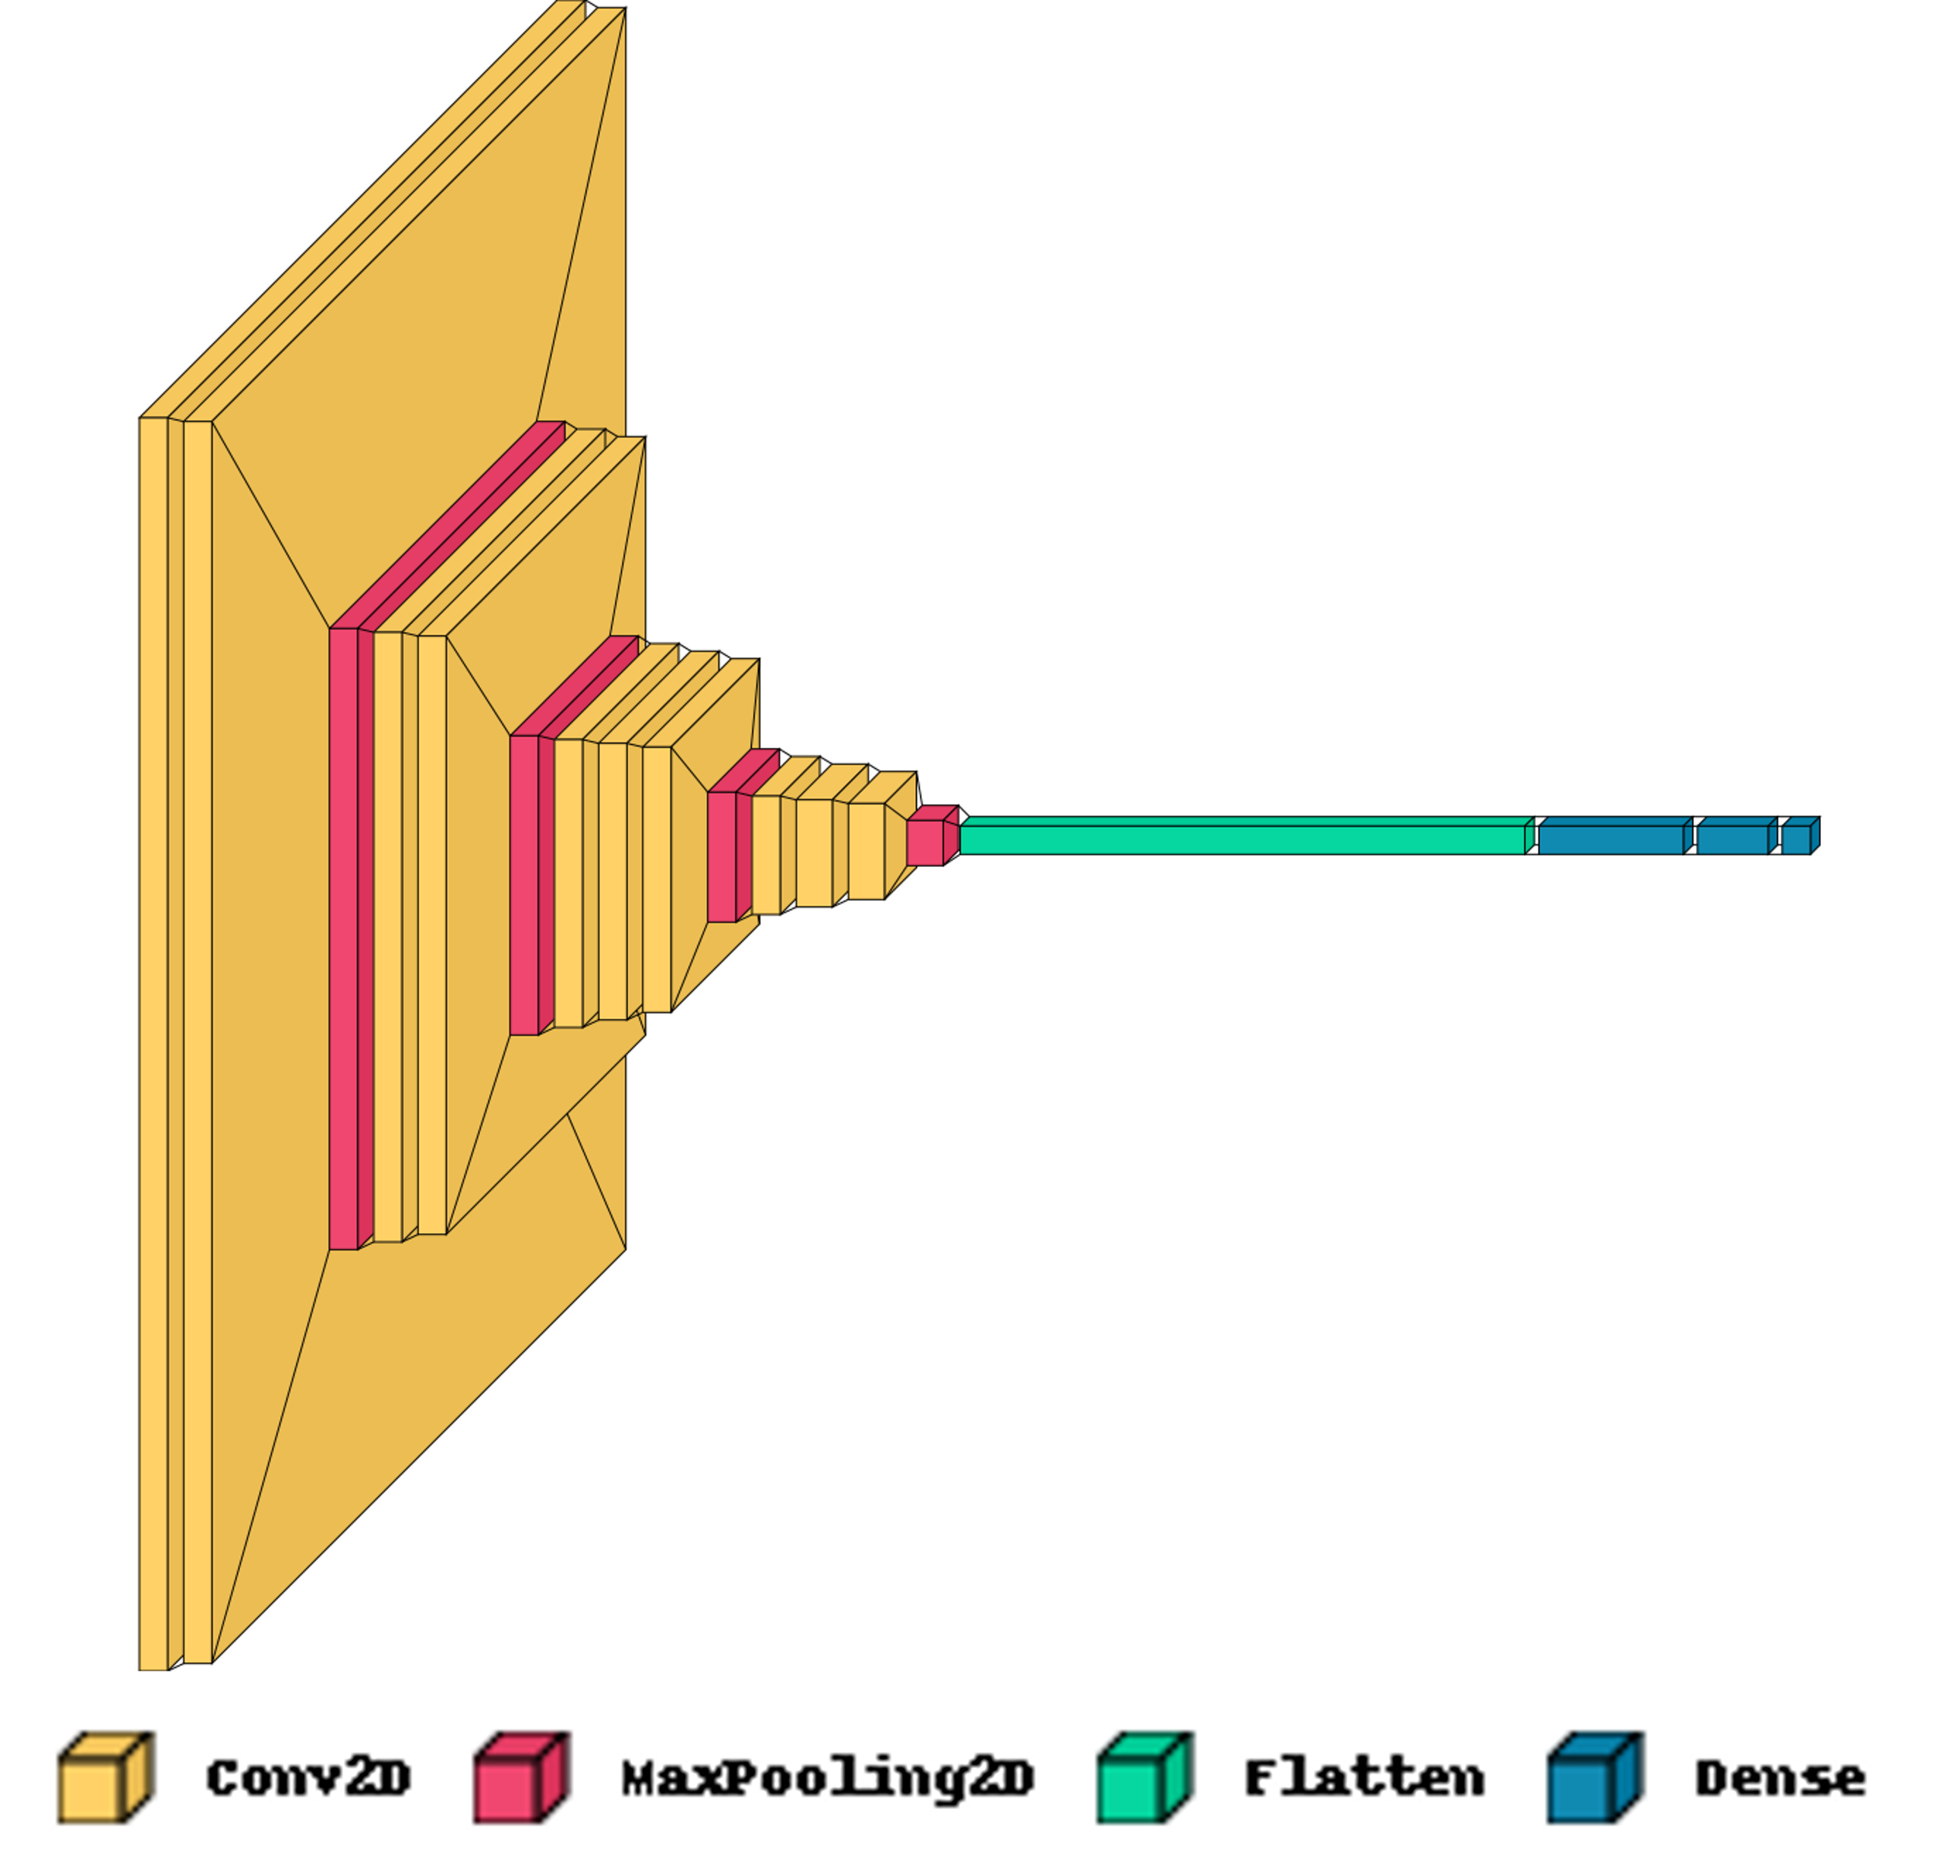
\includegraphics[width=0.4\textwidth]{img/model_dropout_false_batchnorm_false.png}
            \caption{Visualization of our model}
        \end{figure}
    \end{frame}

    
    \begin{frame}{Potential Solution: Dropout}
        \begin{figure}
            \centering
            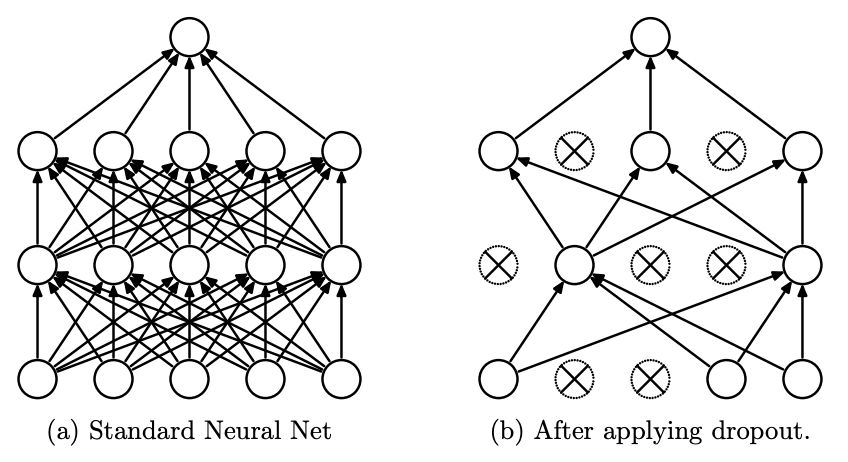
\includegraphics[width=0.6\textwidth]{img/dropout_schema.png}
            \caption{Scheme explaining the principle of Dropout Layers}
        \end{figure}
    \end{frame}


    \begin{frame}{Potential Solution: Batch Normalization}
        \begin{figure}
            \centering
            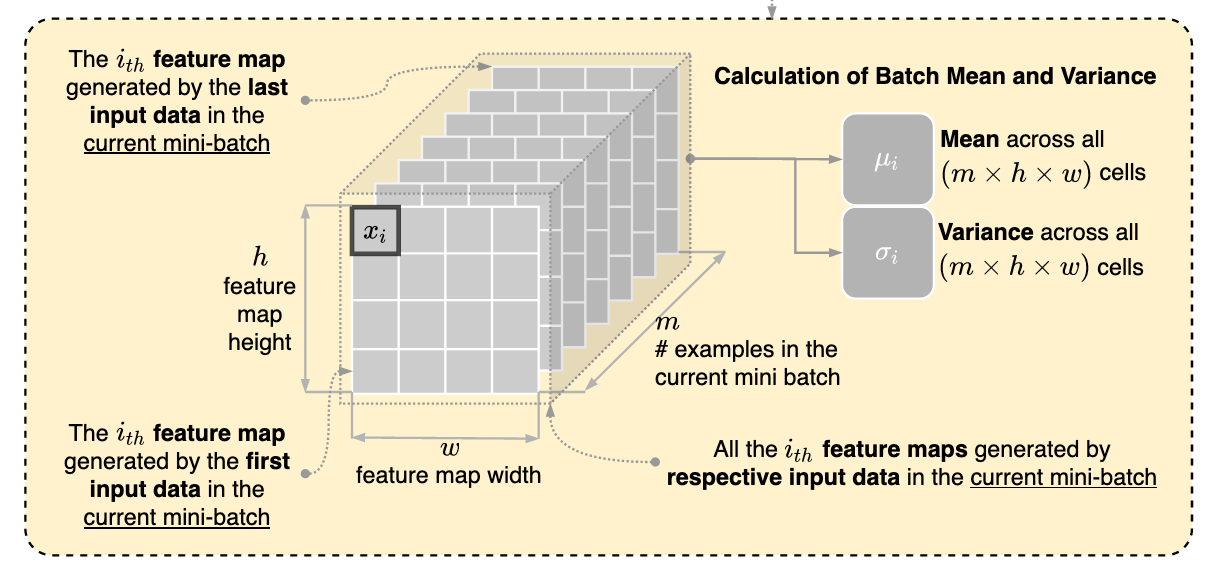
\includegraphics[width=0.8\textwidth]{img/BatchNorm_Schema.png}
            \caption{Scheme explaining the principle of Batch Normalization}
        \end{figure}
    \end{frame}

\section{Experiment} 

\begin{frame}{Model performance without any Regularization}
        \begin{column}{.5\textwidth}
            \begin{figure}
                \centering
                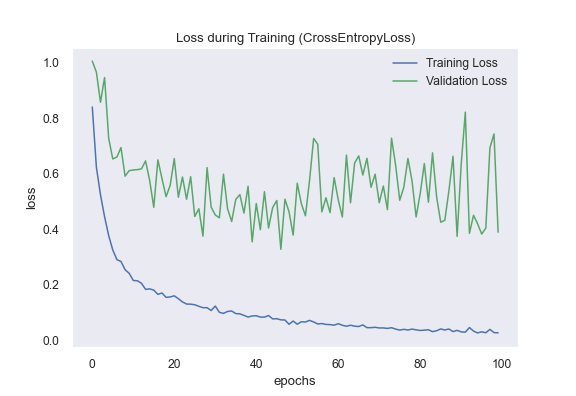
\includegraphics[width=1\textwidth]{img/baptiste_100epoches_val_loss__Dropouts_False__BatchNorm_False.png}
                \caption{Training v Validation Loss}
            \end{figure}
        \end{column}
        \begin{column}{.5\textwidth}
            \begin{figure}
                \centering
                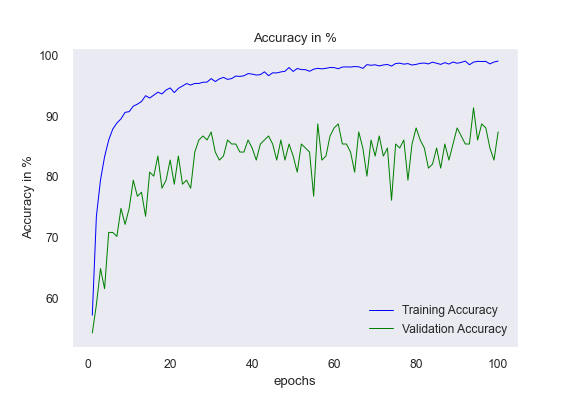
\includegraphics[width=1\textwidth]{img/baptiste_100epoches_train_accuracy__Dropouts_False__BatchNorm_False.png}
                \caption{Training v Validation Accuracy}
            \end{figure}
        \end{column}
    \end{frame}

    \begin{frame}{Model performance without any Regularization}
        \begin{figure}
            \centering
            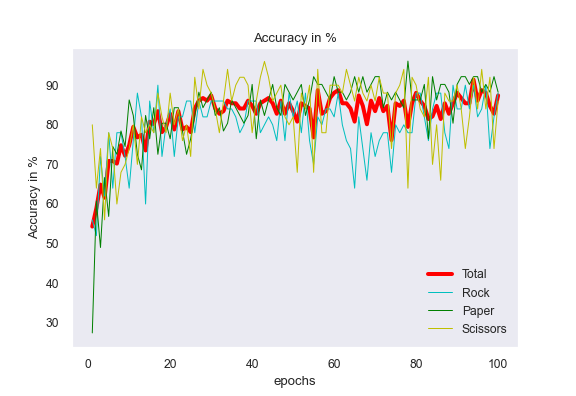
\includegraphics[width=0.6\textwidth]{img/baptiste_100epoches_accuracy__Dropouts_False__BatchNorm_False.png}
            \caption{Validation Accuracy in detail}
        \end{figure}
    \end{frame}

    \begin{frame}{Model performance without any Regularization}
        \begin{figure}
            \centering
            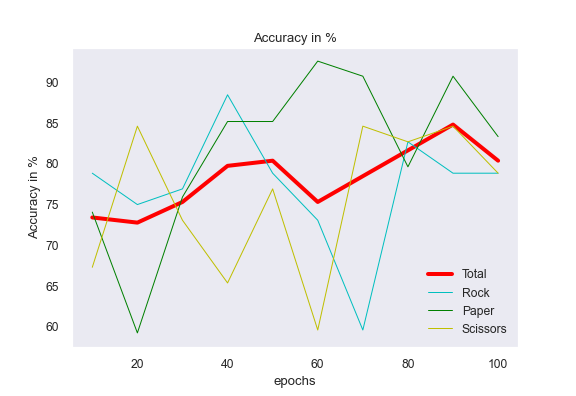
\includegraphics[width=0.6\textwidth]{img/baptiste_100_epoches_test_accuracy__Dropouts_False__BatchNorm_False.png}
            \caption{Testing Accuracy in detail}
        \end{figure}
    \end{frame}

    
    \begin{frame}{Model with Dropout}
        \begin{figure}
            \centering
            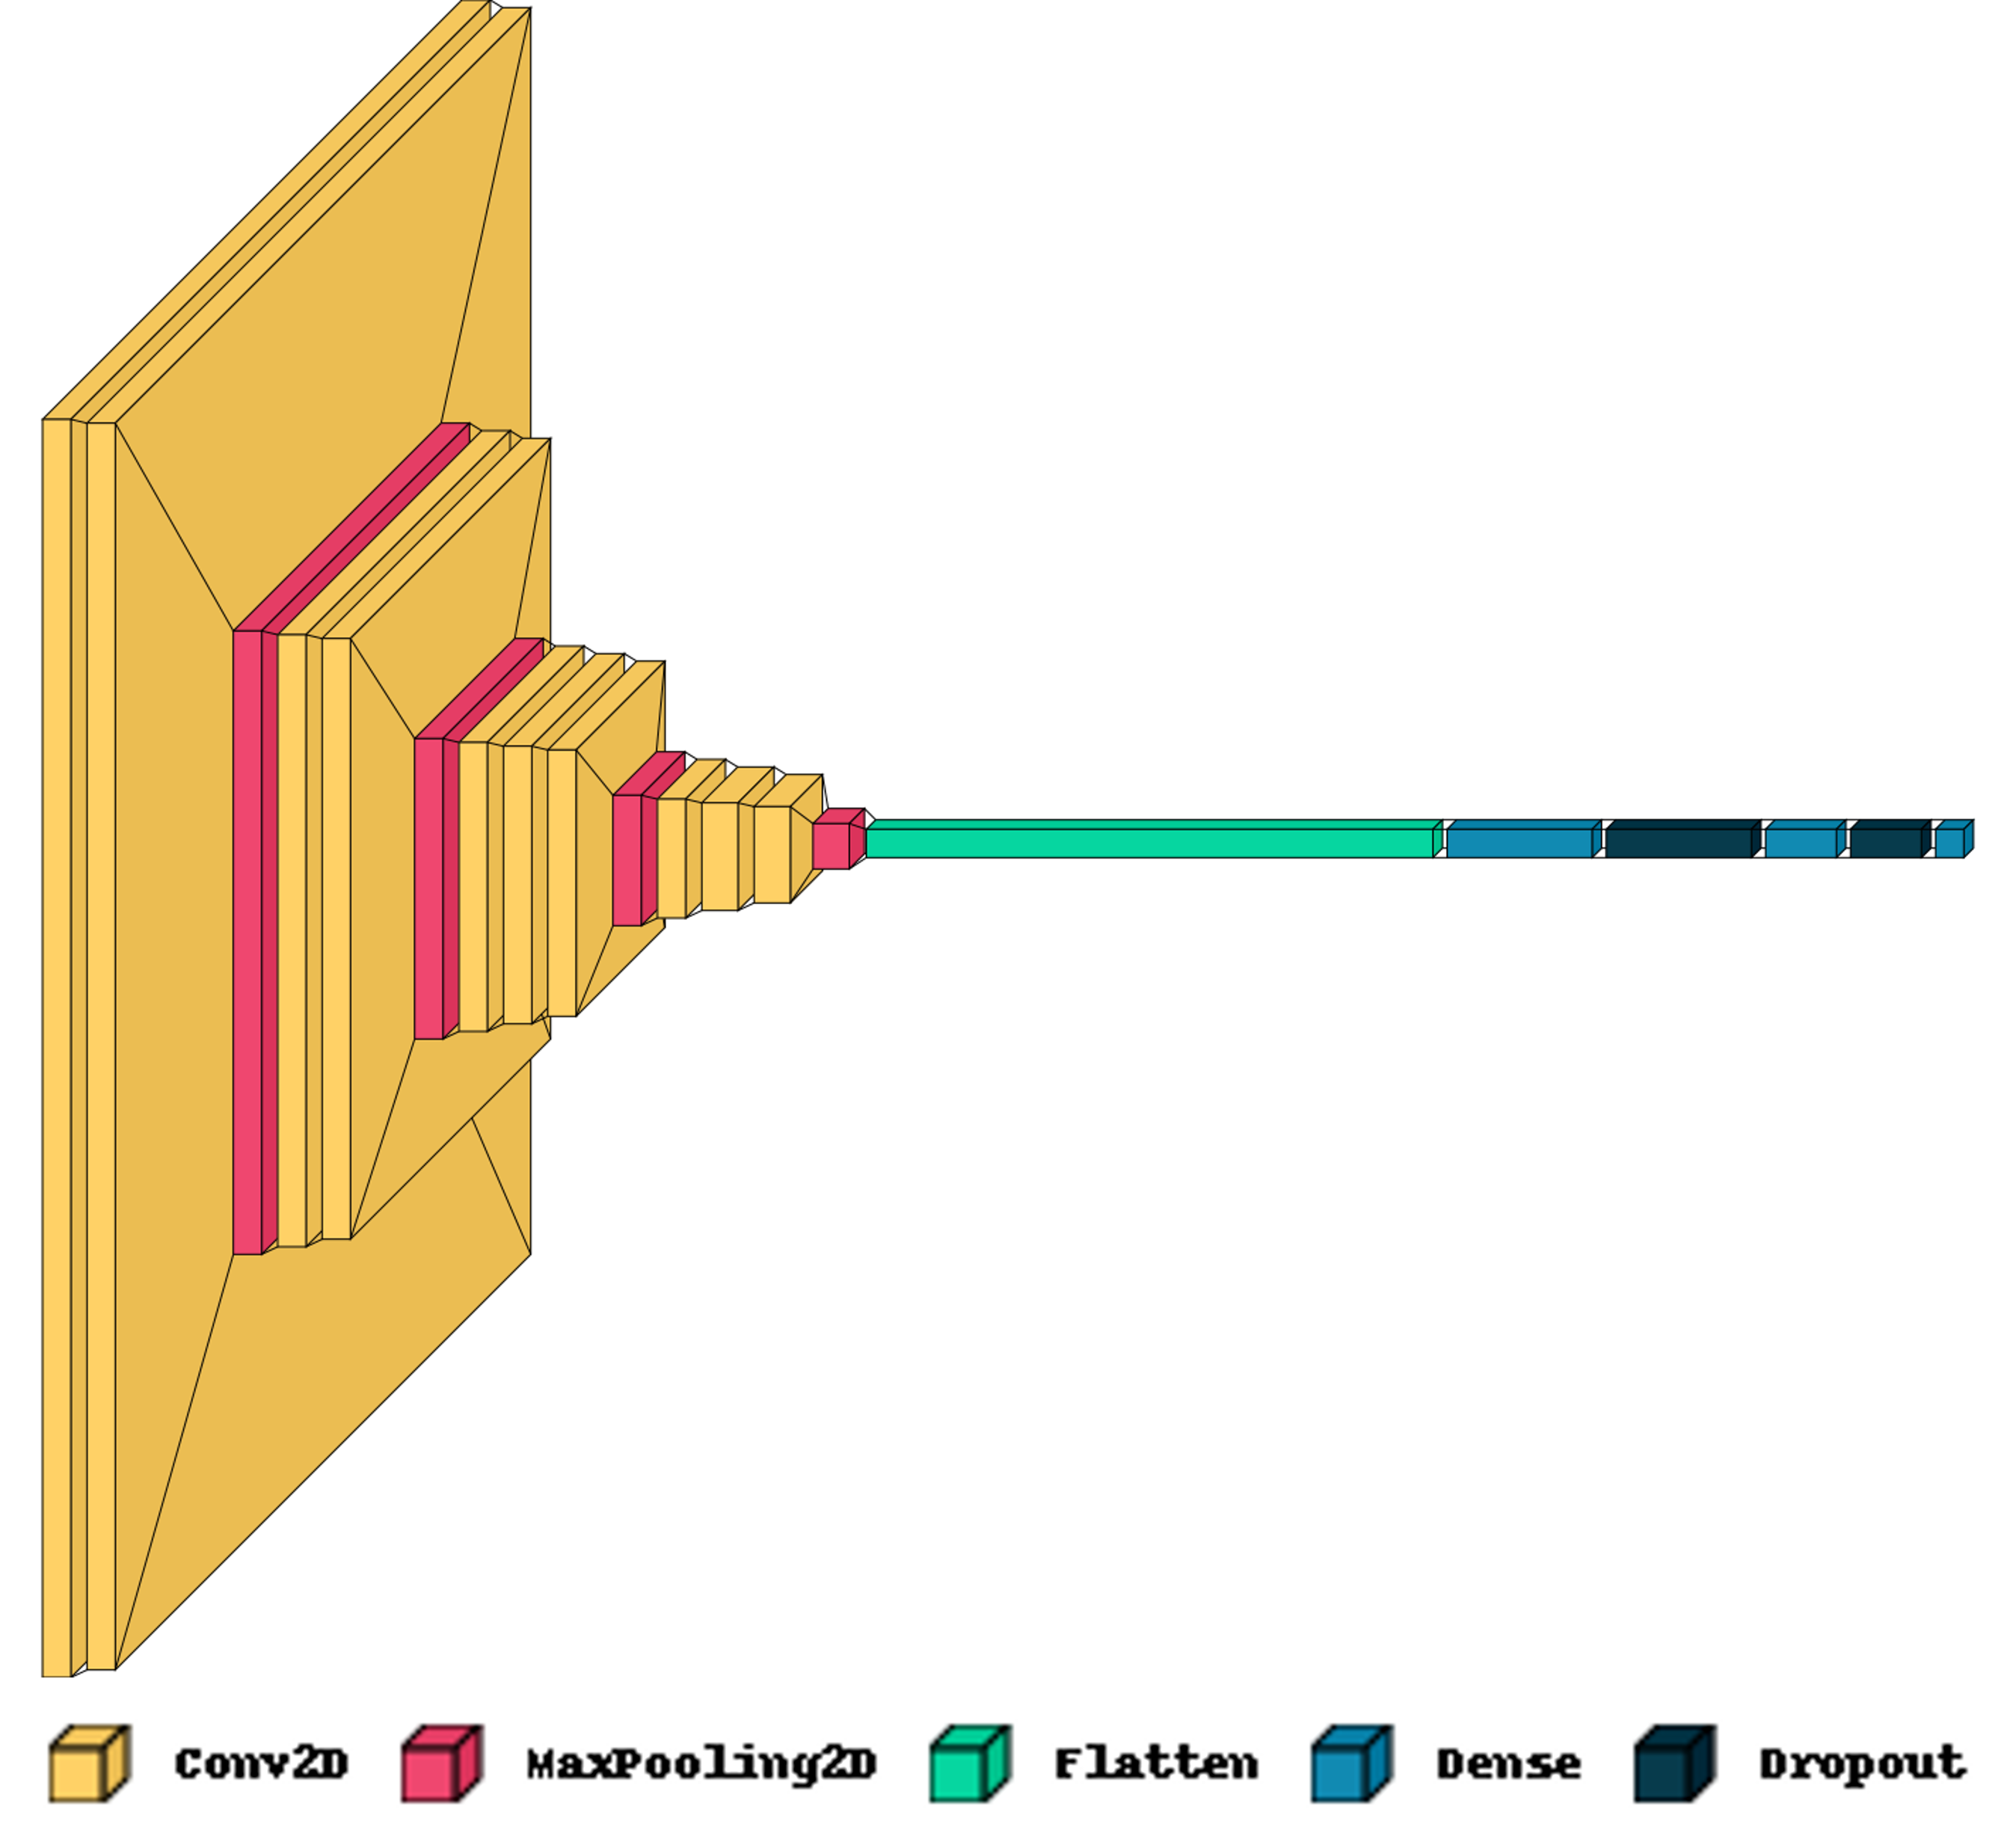
\includegraphics[width=0.4\textwidth]{img/model_dropout_true_batchnorm_false.png}
            \caption{Visualization of our model with Dropout}
        \end{figure}
    \end{frame}


    
    \begin{frame}{Model performance with Dropout}
        \begin{column}{.5\textwidth}
            \begin{figure}
                \centering
                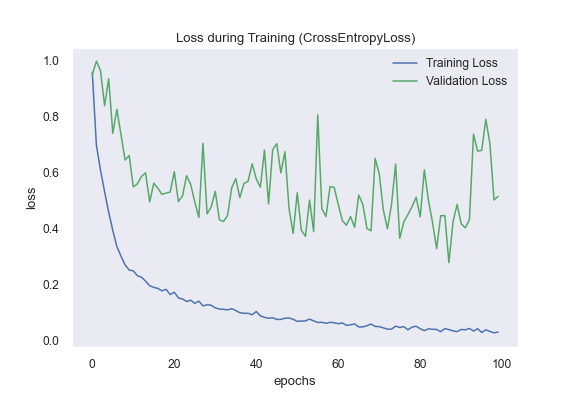
\includegraphics[width=1\textwidth]{img/baptiste_100epoches_val_loss__Dropouts_True__BatchNorm_False.png}
                \caption{Training v Validation Loss}
            \end{figure}
        \end{column}
        \begin{column}{.5\textwidth}
            \begin{figure}
                \centering
                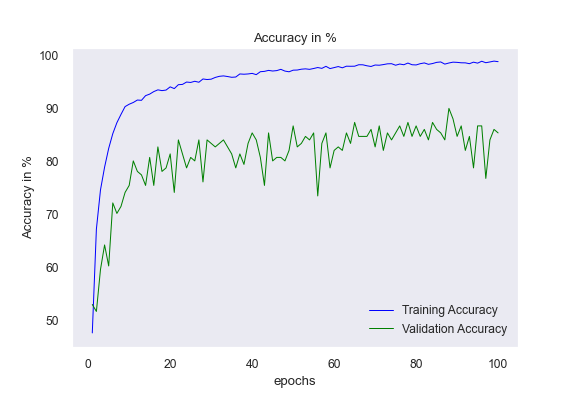
\includegraphics[width=1\textwidth]{img/baptiste_100epoches_train_accuracy__Dropouts_True__BatchNorm_False.png}
                \caption{Training v Validation Accuracy}
            \end{figure}
        \end{column}
    \end{frame}


    \begin{frame}{Model performance with Dropout}
        \begin{figure}
            \centering
            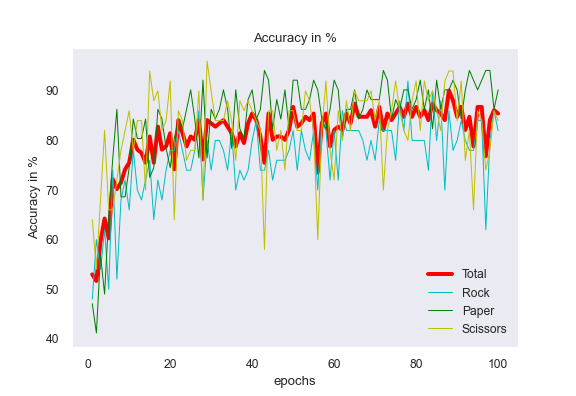
\includegraphics[width=0.6\textwidth]{img/baptiste_100epoches_accuracy__Dropouts_True__BatchNorm_False.png}
            \caption{Validation Accuracy in detail}
        \end{figure}
    \end{frame}

    \begin{frame}{Model performance with Dropout}
        \begin{figure}
            \centering
            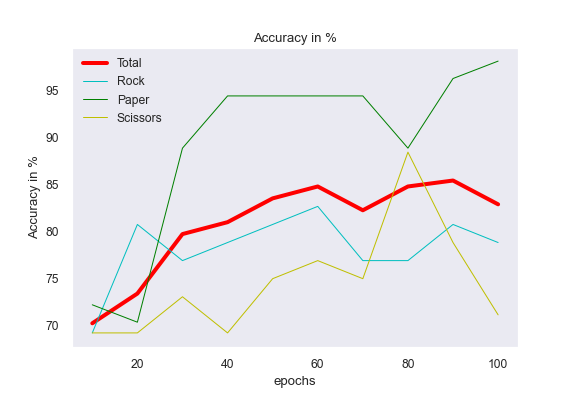
\includegraphics[width=0.6\textwidth]{img/baptiste_100_epoches_test_accuracy__Dropouts_True__BatchNorm_False.png}
            \caption{Testing Accuracy in detail}
        \end{figure}
    \end{frame}


    \begin{frame}{Model with Batch Normalization}
        \begin{figure}
            \centering
            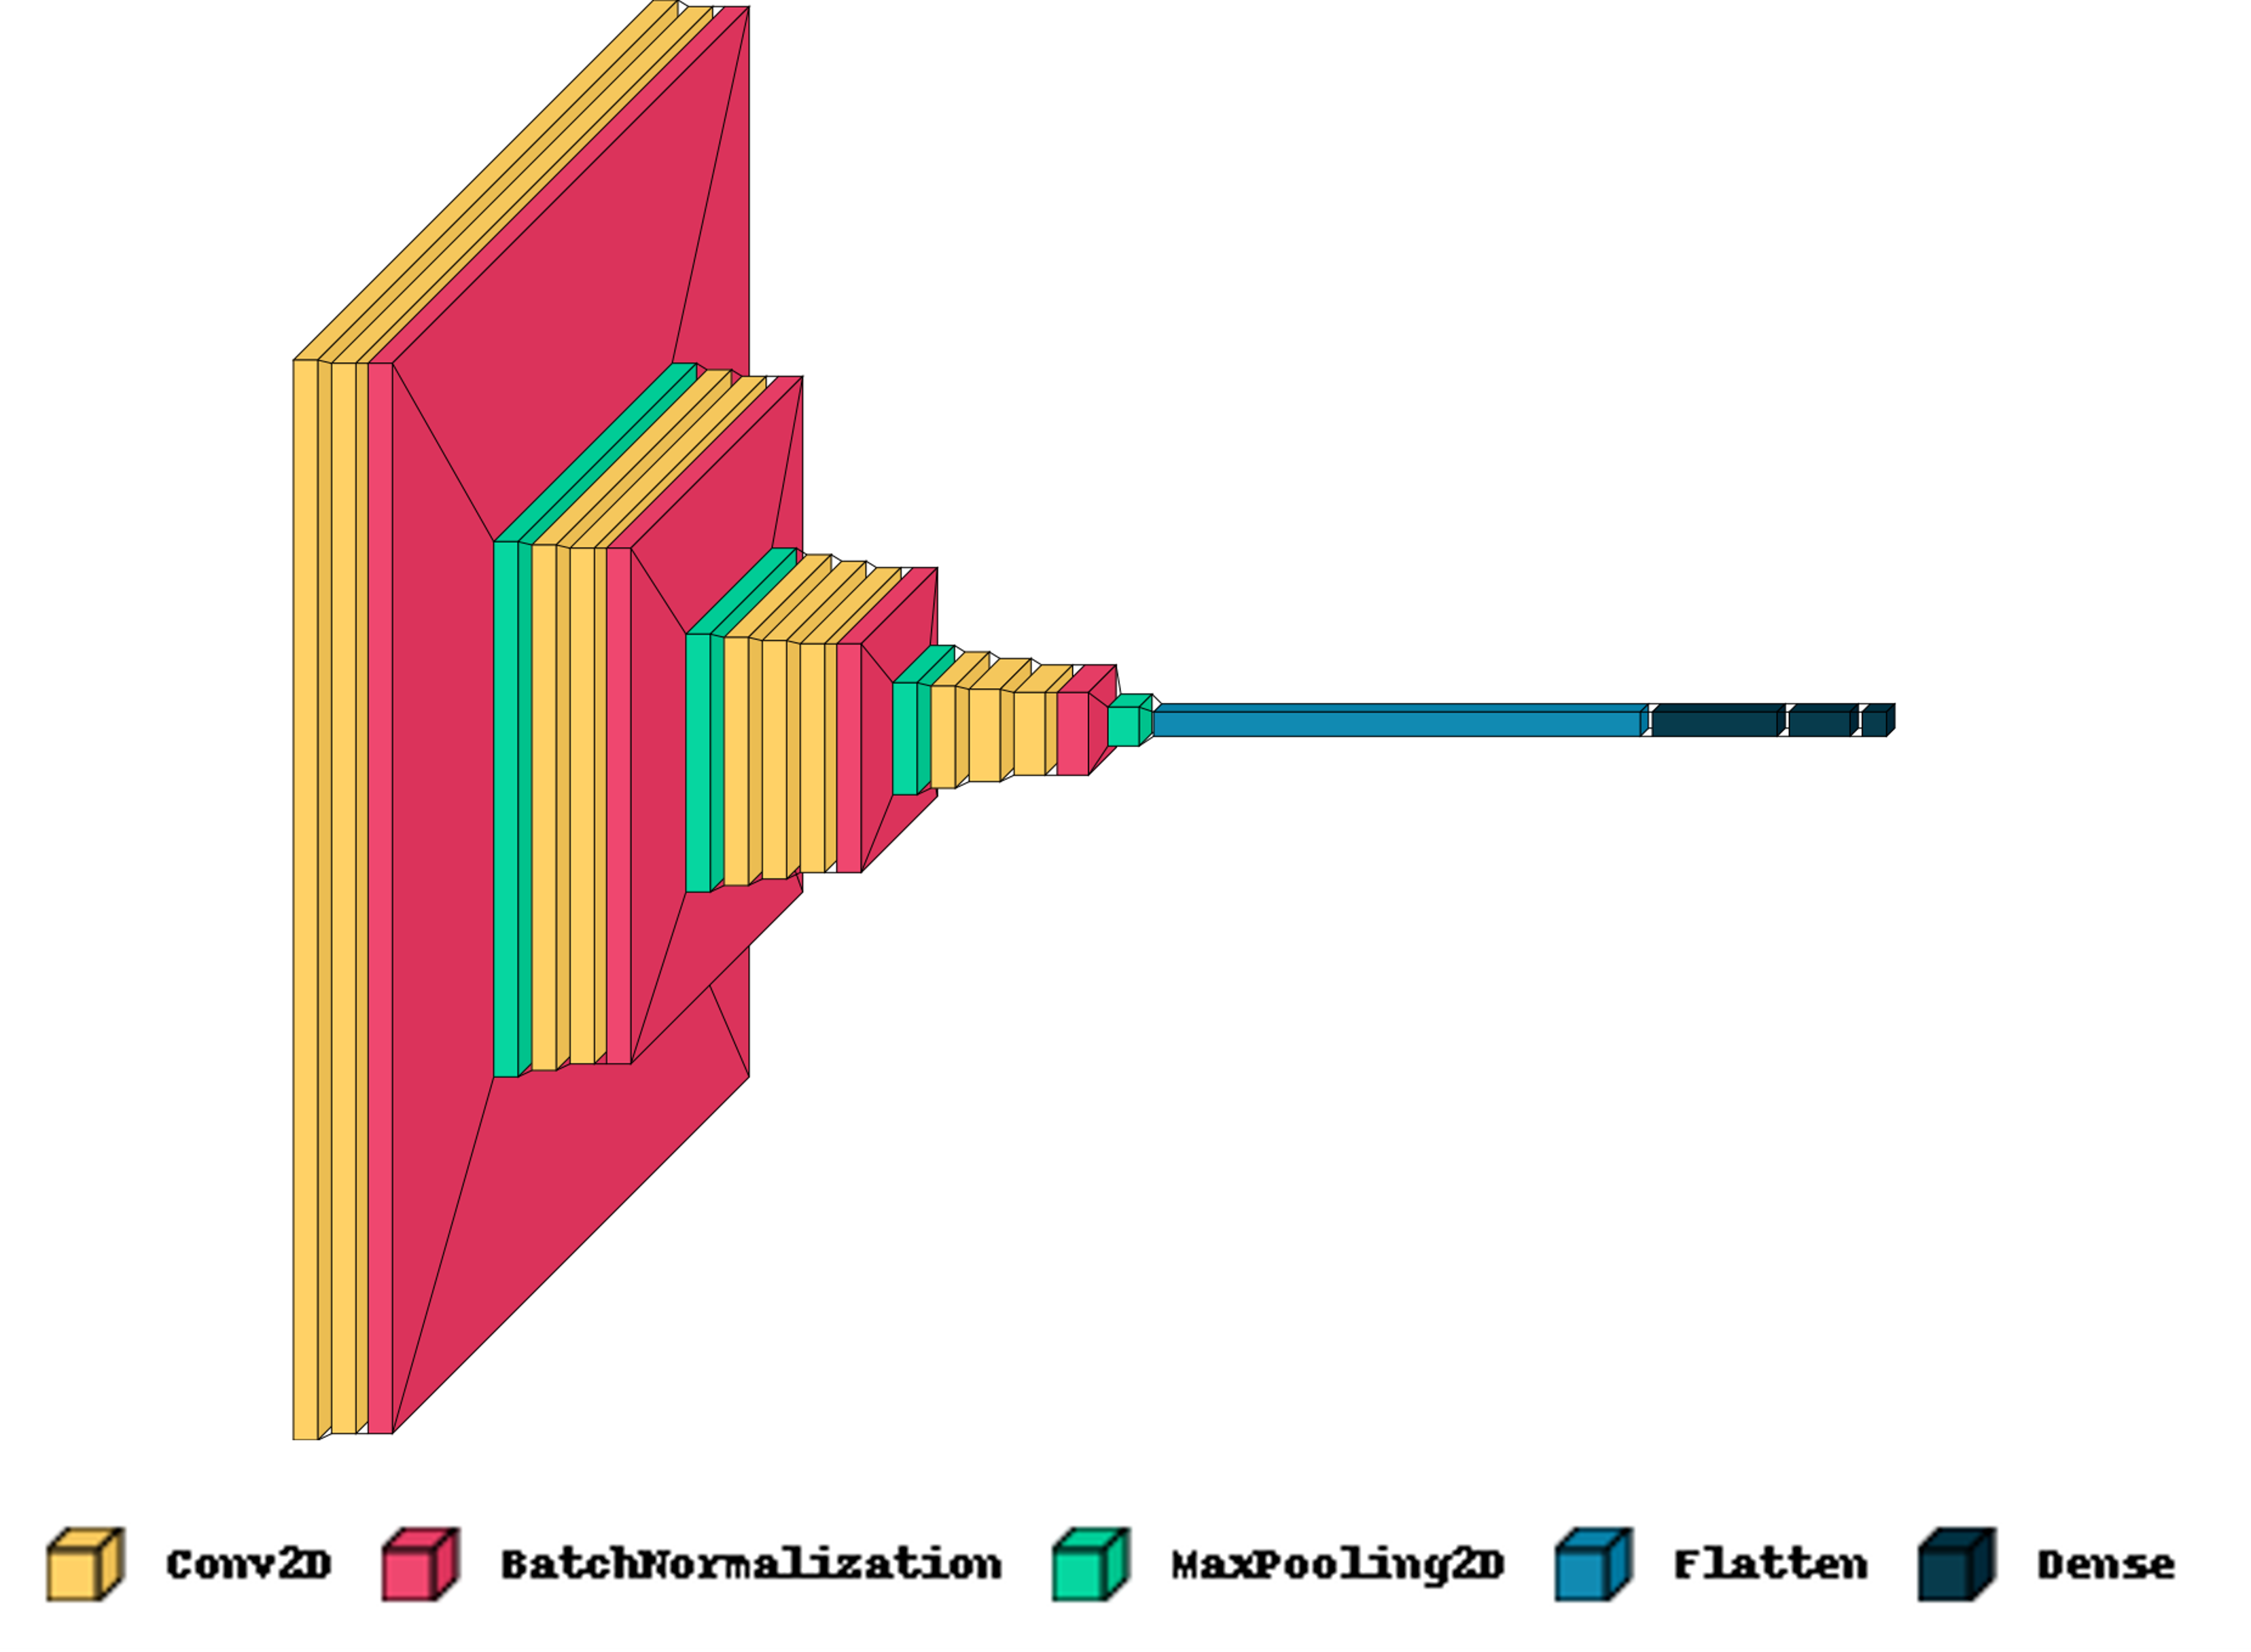
\includegraphics[width=0.4\textwidth]{img/model_dropout_false_batchnorm_true.png}
            \caption{Visualization of our model with Batch Normalization}
        \end{figure}
    \end{frame}

    \begin{frame}{Model performance with Batch Normalization}
        \begin{column}{.5\textwidth}
            \begin{figure}
                \centering
                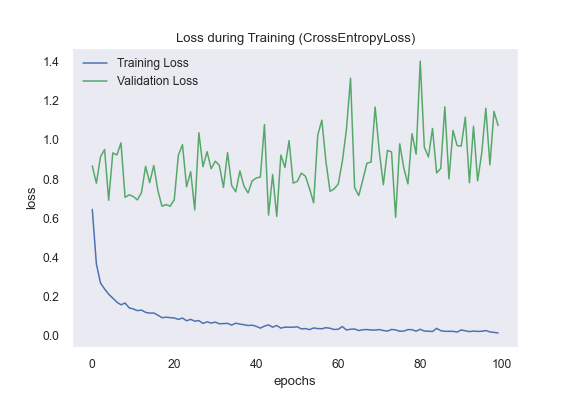
\includegraphics[width=1\textwidth]{img/baptiste_100epoches_val_loss__Dropouts_False__BatchNorm_True.png}
                \caption{Training v Validation Loss}
            \end{figure}
        \end{column}
        \begin{column}{.5\textwidth}
            \begin{figure}
                \centering
                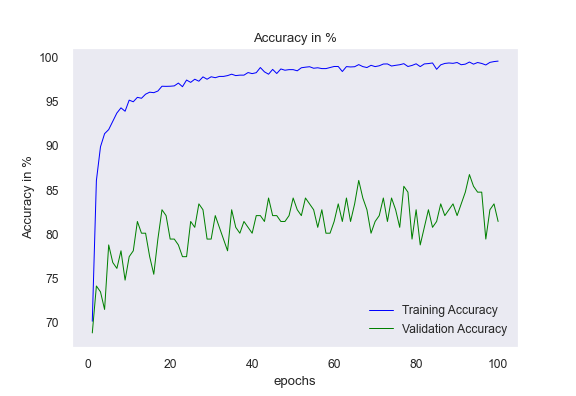
\includegraphics[width=1\textwidth]{img/baptiste_100epoches_train_accuracy__Dropouts_False__BatchNorm_True.png}
                \caption{Training v Validation Accuracy}
            \end{figure}
        \end{column}
    \end{frame}

    \begin{frame}{Model performance with Batch Normalization}
        \begin{figure}
            \centering
            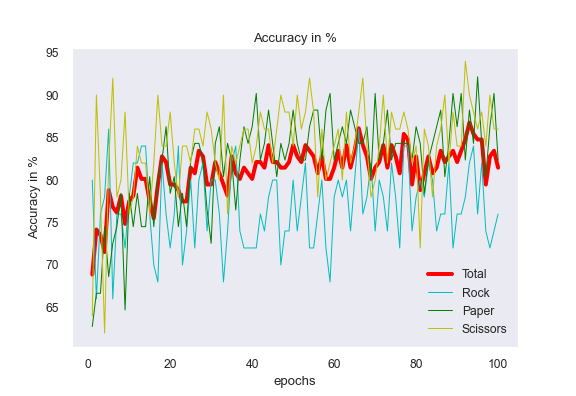
\includegraphics[width=0.6\textwidth]{img/baptiste_100epoches_accuracy__Dropouts_False__BatchNorm_True.png}
            \caption{Validation Accuracy in detail}
        \end{figure}
    \end{frame}

    \begin{frame}{Model performance with Batch Normalization}
        \begin{figure}
            \centering
            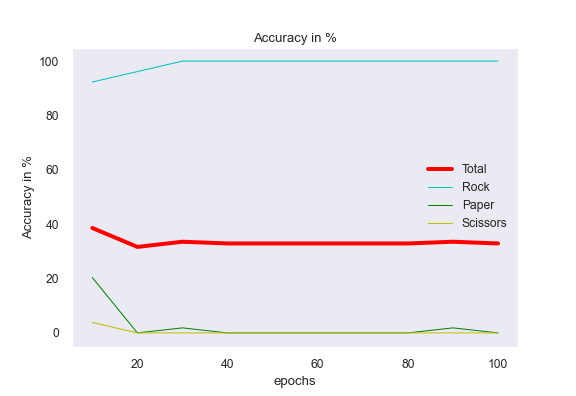
\includegraphics[width=0.6\textwidth]{img/baptiste_100_epoches_test_accuracy__Dropouts_False__BatchNorm_True.png}
            \caption{Testing Accuracy in detail}
        \end{figure}
    \end{frame}


    \begin{frame}{Model with both Dropout \& Batch Normalization}
        \begin{figure}
            \centering
            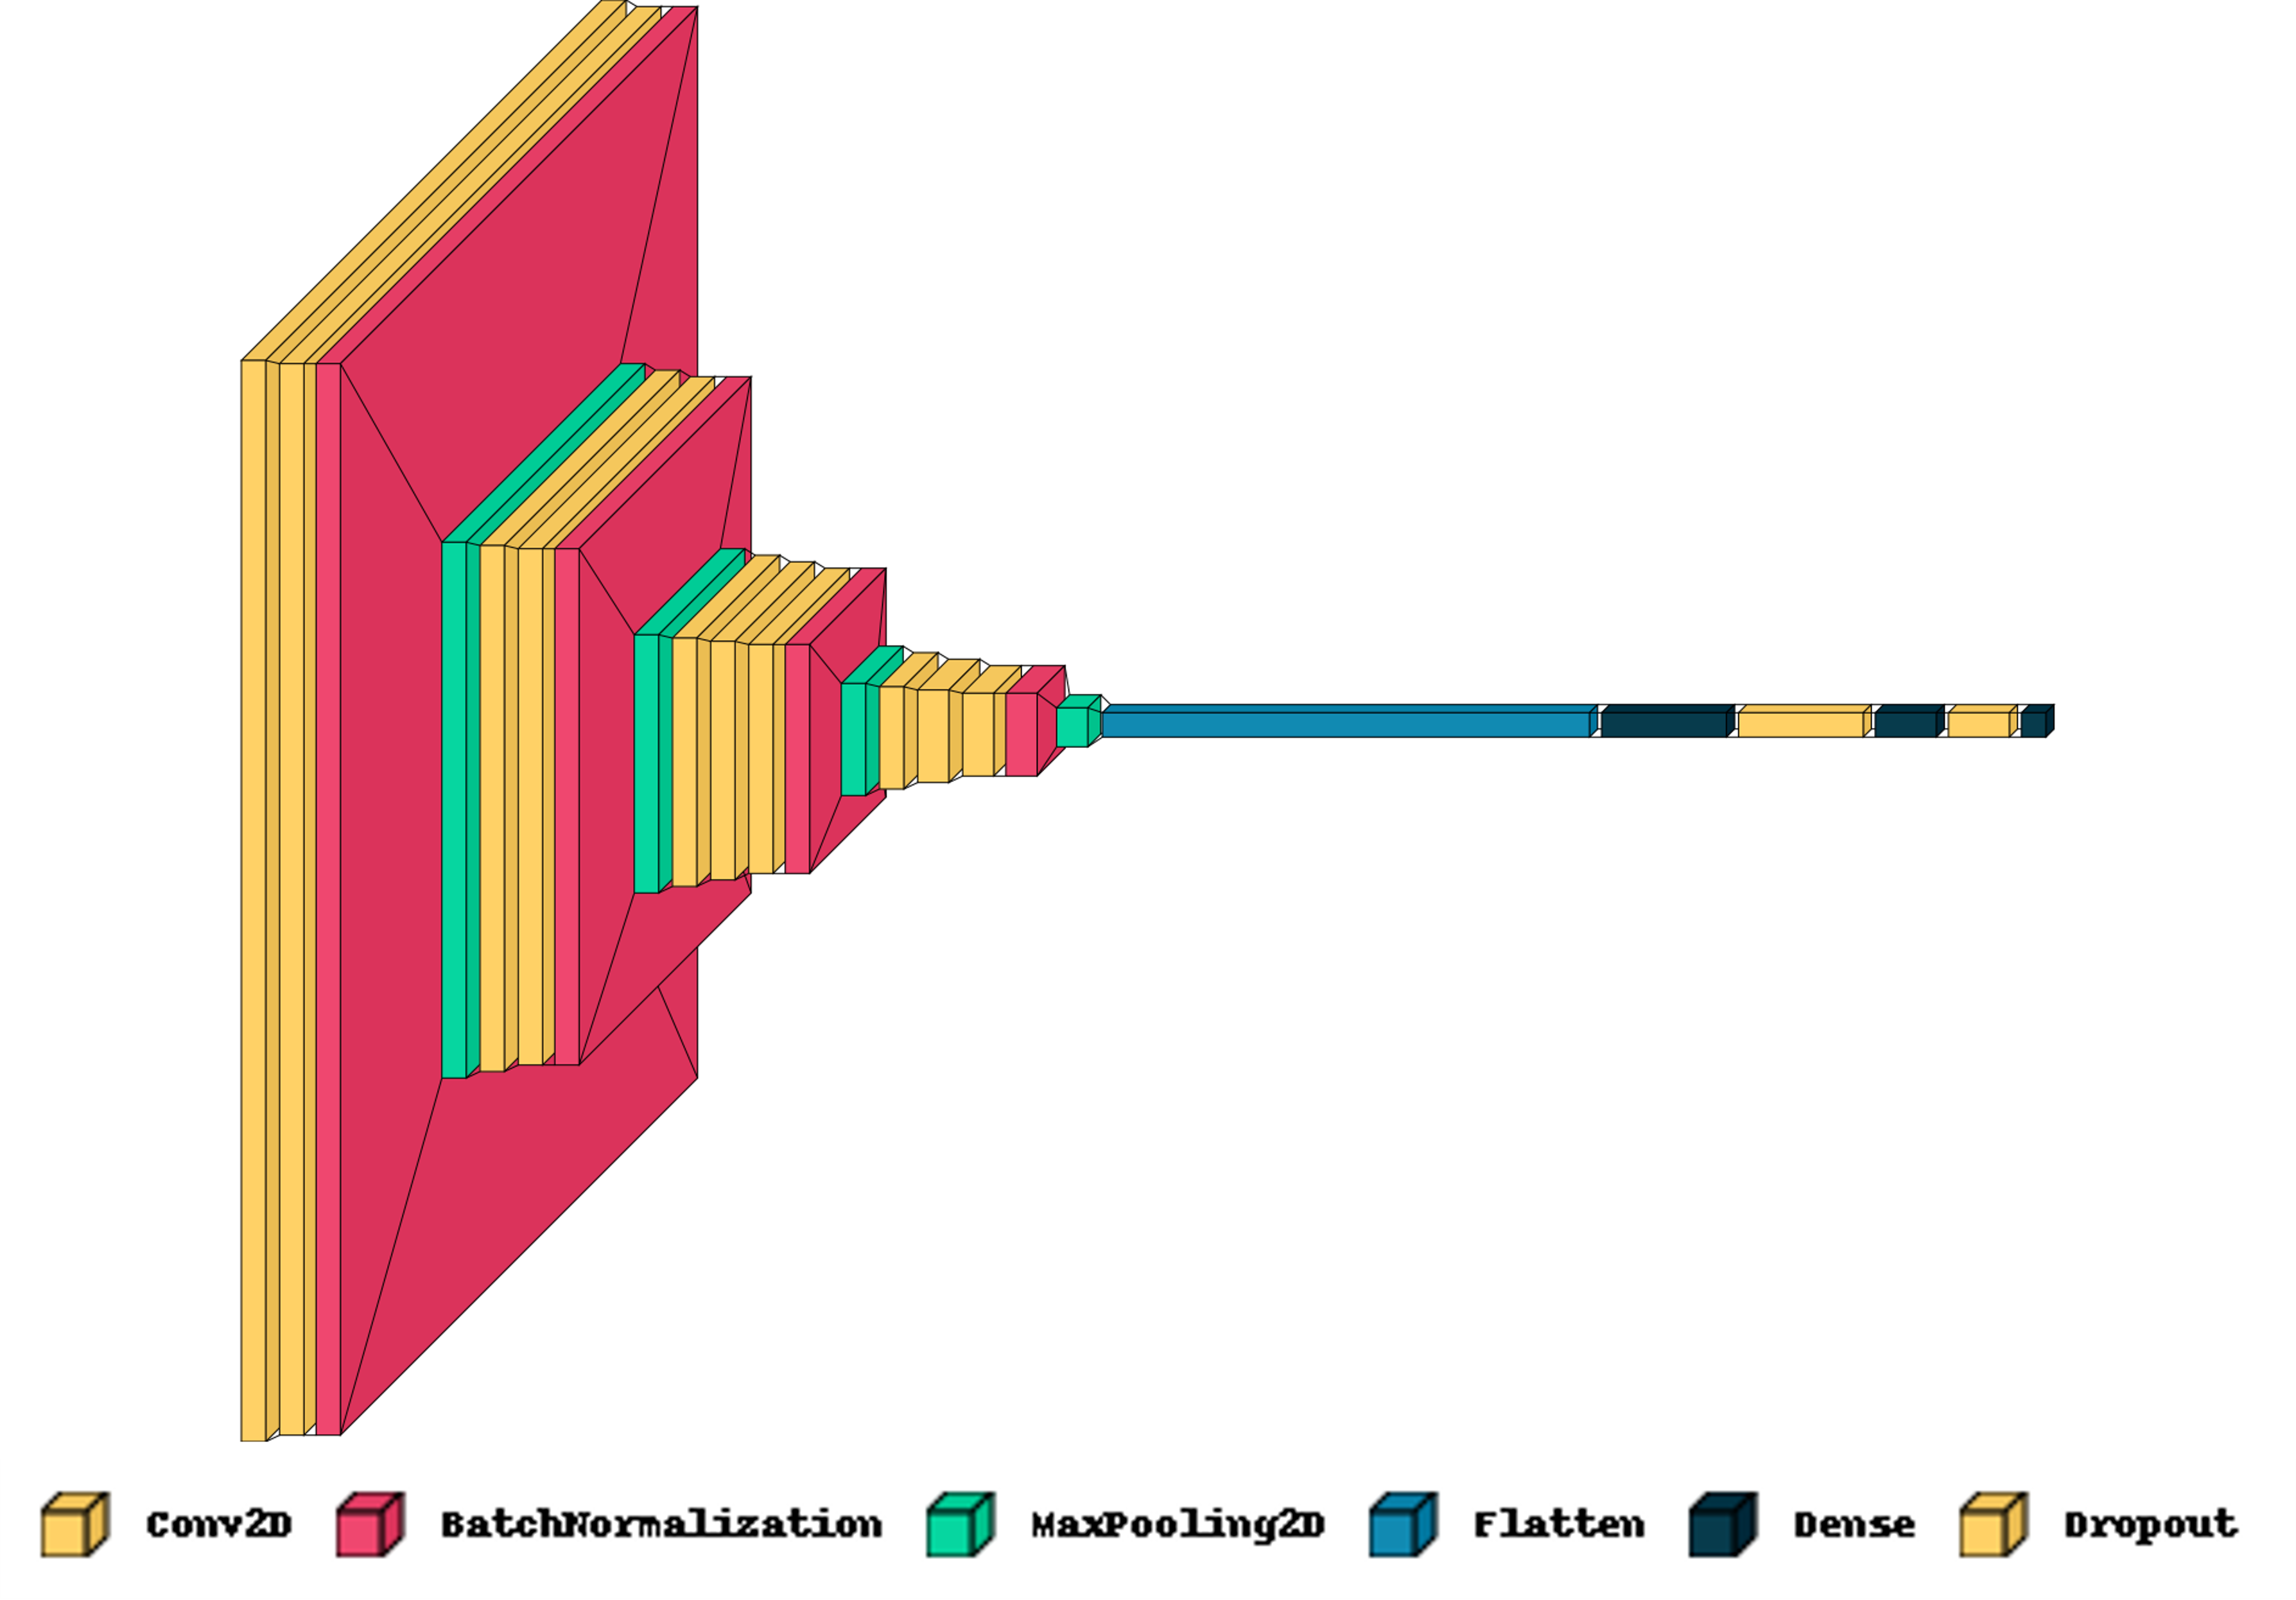
\includegraphics[width=0.4\textwidth]{img/model_dropout_true_batchnorm_true.png}
            \caption{Visualization of our model with both Dropout \& Batch Normalization}
        \end{figure}
    \end{frame}

    
    \begin{frame}{Model performance with both Dropout \& Batch Normalization}
        \begin{column}{.5\textwidth}
            \begin{figure}
                \centering
                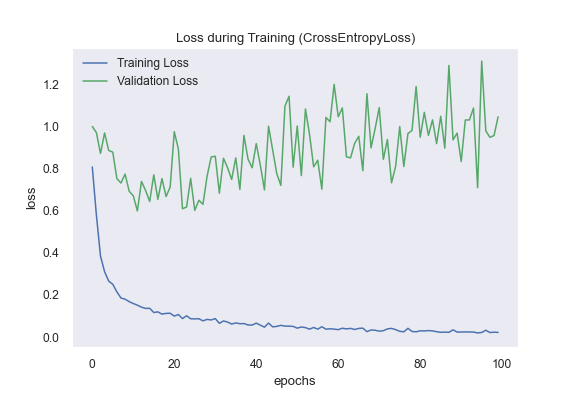
\includegraphics[width=1\textwidth]{img/baptiste_100epoches_val_loss__Dropouts_True__BatchNorm_True.png}
                \caption{Training v Validation Loss}
            \end{figure}
        \end{column}
        \begin{column}{.5\textwidth}
            \begin{figure}
                \centering
                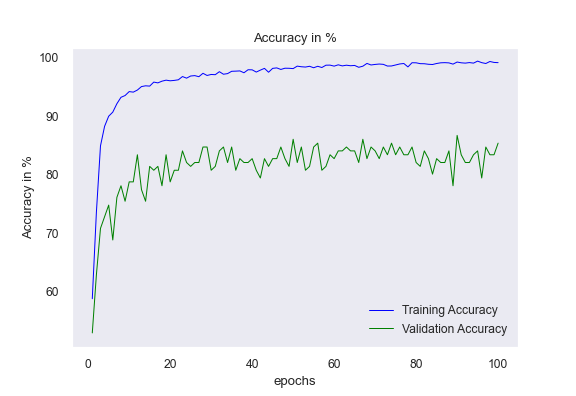
\includegraphics[width=1\textwidth]{img/baptiste_100epoches_train_accuracy__Dropouts_True__BatchNorm_True.png}
                \caption{Training v Validation Accuracy}
            \end{figure}
        \end{column}
    \end{frame}

    \begin{frame}{Model performance with both Dropout \& Batch Normalization}
        \begin{figure}
            \centering
            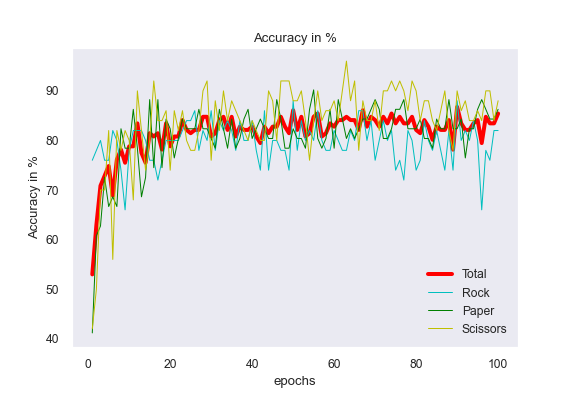
\includegraphics[width=0.6\textwidth]{img/baptiste_100epoches_accuracy__Dropouts_True__BatchNorm_True.png}
            \caption{Validation Accuracy in detail}
        \end{figure}
    \end{frame}

    \begin{frame}{Model performance with both Dropout \& Batch Normalization}
        \begin{figure}
            \centering
            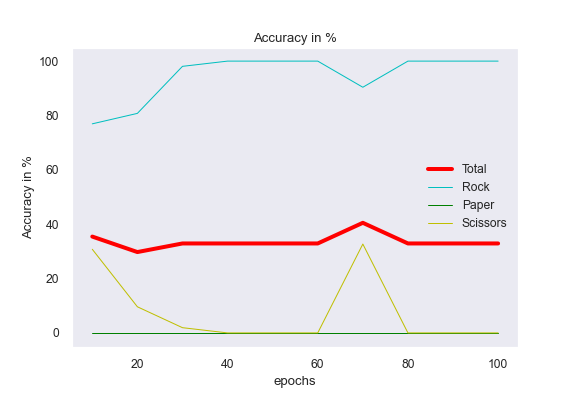
\includegraphics[width=0.6\textwidth]{img/baptiste_100_epoches_test_accuracy__Dropouts_True__BatchNorm_True.png}
            \caption{Testing Accuracy in detail}
        \end{figure}
    \end{frame}
    

    \begin{frame}{Comparison between the four cases}
        \begin{figure}
            \centering
            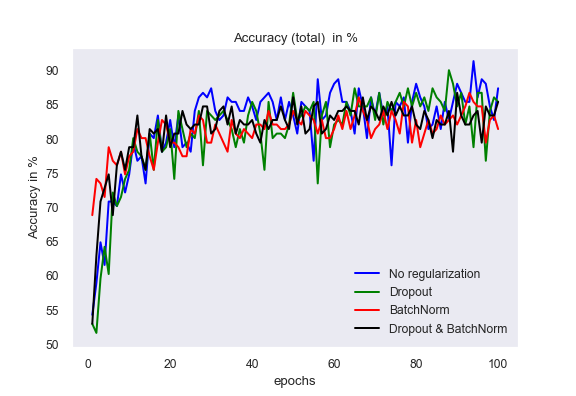
\includegraphics[width=0.6\textwidth]{img/baptiste_val_accuracies_comparison.png}
            \caption{Comparison between all Validation Accuracies}
        \end{figure}
    \end{frame}


    \begin{frame}{Comparison between the four cases}
        \begin{figure}
            \centering
            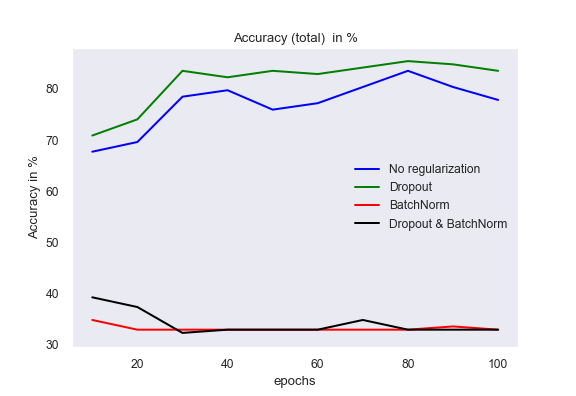
\includegraphics[width=0.6\textwidth]{img/baptiste_test_accuracies_comparison.png}
            \caption{Comparison between all Testing Accuracies}
        \end{figure}
    \end{frame}

    \begin{frame}{Final results (with Dropout)}
        \begin{table}[]
            \begin{tabular}{@{}lllll@{}}
            \toprule
            \multicolumn{1}{c}{} & Rock & Paper & Scissors & Total \\ \midrule
            Val Set                     & 86,00\%  & 90,20\%   & 78,00\%      & 84,77\%   \\
            Test Set                        & 78,85\%  & 98,15\%   & 71,15\%      & 82,91\%  \\
            \bottomrule
            \end{tabular}
            \caption{Accuracies on Val Set and Test Set for the Leaderboard}
        \end{table}
    \end{frame}


% finally our last stuff
\appendix
{\nologo
	\begin{frame}[standout]
		Thank you!
	\end{frame}

    
	\begin{frame}[allowframebreaks]{References}
	
	\bibliographystyle{ieeetr}
  	\bibliography{references}
  	

	\end{frame}
}
\end{document}